% Section 6 (OUTLINE.md §6; 3 pages). Code anchors are at main-repo commit d58c9ef
% (branch phase-2-cr-acceptance), which contains D-34 (b9c66c0) and the CR acceptance config
% (c823d20). Re-anchor on the release commit (TODO 20).
\section{Forecasts, the predictive contract and the verdict engine}\label{sec:evaluation}\label{sec:forecasts}

Both engines return the same object, a \code{ForecastResult}, and everything downstream of a fit
(scores, backtests, tests and verdicts) reads only that object.
None of the scoring rules, tests or estimators below is new; what the package adds is one contract
that makes them available, with their Monte Carlo error, to the compositions of
\cref{sec:framework} (the path-integrated estimator of \cref{sec:eval-tail} to MCMC forecasts
only).

\subsection{Joint path simulation}\label{sec:eval-paths}

Let $s = 1, \dots, S$ index forecast draws and $T$ be the forecast origin.
For each selected posterior draw, the MCMC engine first simulates the future log variances,
including future outlier and Student-$t$ scales; $\lambda^{\mathrm{eff}}_{s,T+h}$ denotes the
effective variances (with those scales) and $\lambda^{\mathrm{pers}}_{s,T+h}$ the persistent ones.
It then runs over $h = 1, \dots, H$, building $x_{s,T+h}$ from the simulated path:
\begin{equation}\label{eq:forecast-recursion}
  m_{s,h} = B_s'\, x_{s,T+h},\qquad
  L_{s,h} = A_s^{-1}\operatorname{diag}\bigl(\lambda^{\mathrm{eff}}_{s,T+h}\bigr)^{1/2},\qquad
  y_{s,T+h} = m_{s,h} + L_{s,h}\,\varepsilon_{s,h},
\end{equation}
with $\varepsilon_{s,h} \sim N(0, I_n)$ and $B_s' = A_s^{-1}\Gamma_s$ in structural form ($B_s = \Pi_s$
in reduced form).
% [V] src/rai_bvar/engines/mcmc/forecast.py module docstring l.12-14 at d58c9ef (structural: A^{-1}Γx; reduced: Π'x; m = B'x)
Because $A_s$ is unit lower triangular, $L_{s,h}$ is the Cholesky factor of the conditional
covariance at no extra cost, and $y_{T+h} \mid \theta_s, y_{s,T+1:T+h-1}, \lambda_{s,T+h} \sim
N(m_{s,h}, L_{s,h}L_{s,h}')$ holds exactly.
The analytic engine draws $(B, \Sigma)$ from the NIW posterior and uses
$L = \operatorname{chol}(\Sigma)$, scaled by the future Lenza--Primiceri factor when that treatment
is active \citep{lenza2022estimate}.
Forecast draws are evenly spaced stored draws of each chain, and their shocks are keyed by
(forecast seed, chain, kept-draw index), so a forecast computed inside the sampling loop equals the
one computed afterwards from the stored draws to $10^{-12}$.
% [V] tests/mcmc/forecast/test_forecast_core.py::test_in_loop_forecast_equals_post_hoc_constant (rtol=atol=1e-12); ::test_in_loop_forecast_equals_post_hoc_sv (slow)
Impulse responses use $\Phi_0 = I$, $\Phi_j = \sum_{l=1}^{\min(j,p)} A_l\Phi_{j-l}$ with $A_l$ the
reduced-form lag matrices; unit-shock responses $\Phi_j A^{-1}$ are date-free, while
one-standard-deviation responses depend on the date and use the persistent variance by default;
the forecast error variance decomposition is computed from the responses.
% [V] tests/mcmc/forecast/test_irf_mcmc.py::test_irf_equals_direct_phi_ainv_lambda, ::test_unit_shock_irf_is_phi_ainv_and_date_free; FEVD: tests/unit/test_irf.py::test_fevd_matches_forecast_error_covariance

\subsection{The predictive contract}\label{sec:eval-contract}

A \code{ForecastResult} wraps an \pkg{xarray} dataset \citep{hoyer2017xarray} with the fields
\code{paths} (joint paths on the transformed scale), \code{paths\_level} (their pathwise inverse
to levels, never applied to quantiles), \code{cond\_mean} ($m_{s,h}$) and \code{cond\_chol}
($L_{s,h}$), indexed by chain, draw, horizon and variable, and attributes for the origin, model,
engine, spec and spec hash, transformation codes, seed, convergence flag and warnings.
MCMC forecasts also record the variable ordering and sampler settings; analytic forecasts carry
the ordering only as the order of the \code{variable} coordinate.
% dossier 02 §15 D15 (SPEC↔code discrepancy; TODO 18)
The contract has three invariants: $L_{s,h}^{-1}(\code{paths} - \code{cond\_mean})$ is iid
$N(0, I)$; each draw is one joint path across horizons and variables; and stacking chains and draws
is chain-major (\cref{tab:TabC1} in \cref{app:algorithms}).
They are tested for every registered benchmark and analytic-engine model and for 12 MCMC
compositions, eight structural and four reduced-form.
% [V] tests/contract/test_forecast_contract.py (REGISTERED_MODELS: RandomWalk, OLSVAR and the conjugate BVARs), tests/contract/test_forecast_contract_mcmc.py over tests/mcmc/forecast/mcmc_fits.py::COMPOSITIONS (l.128-141 at d58c9ef)
Reduced form $\times$ SV($t$), SV(outliers, $t$) and SV(rw) are not among them; the last is the
primary arm of the replication in \cref{sec:cr}.
\todo{TODO 3: row~18, \code{reduced_sv_rw} (reduced form $\times$ SV(rw)), and a \code{reduced-SV(rw)} contract fit were committed in 7f410dc, after the acceptance commit c823d20; the SV(rw, $t$) variant is still not covered. If the release commit includes it, update this sentence (13 compositions) and the coverage statements of \cref{sec:validation-coverage,sec:replication-caveats,sec:limitations}.}
Accelerator variables may ride along and are never contract fields: MCMC forecasts attach a
factored form of $L_{s,h}$, the transitory parameters and, since D-34, each draw's lag matrices
(\code{lag\_coefs}).

\subsection{The Rao--Blackwellised log predictive density}\label{sec:eval-lpd}

The default estimator (SPEC~\S7) is the mixture of the conditional Gaussian densities,
\begin{equation}\label{eq:rb-lpd}
  \log\hat p_h(y) = \operatorname{logsumexp}_s \log N\bigl(y;\, m_{s,h},\, L_{s,h}L_{s,h}'\bigr) - \log S ,
\end{equation}
so no kernel density estimate is needed; mixture log scores of this kind are standard
\citep{geweke2010comparing,kruger2021predictive}.
A leading block $\{1, \dots, j\}$ of the ordering uses $L_{s,h}[1{:}j, 1{:}j]$, and any other
subset factors the selected rows of $L_{s,h}$ by QR, so marginal scores are exact.
% [V] tests/mcmc/forecast/test_lpd_mcmc.py::test_factored_lpd_equals_cond_chol_lpd, ::test_non_leading_subsets_use_the_qr_factor
With weights $w_s = \exp(\log p_s - \max_r \log p_r)$, the reported Monte Carlo standard error is
the delta-method value
\begin{equation}\label{eq:mcse}
  \widehat{\mathrm{se}}\bigl(\log\hat p_h\bigr) = \frac{\operatorname{sd}(w)}{\sqrt S\,\bar w}
  \times \sqrt{S/\widehat{\mathrm{ESS}}(w)} ,
\end{equation}
with the sample standard deviation; the second factor, with the ESS of the weights over chains and
draws, applies to MCMC forecasts only and is 1 when that ESS is undefined.
% [V] src/rai_bvar/forecast/result.py l.325-338 at d58c9ef (w.std(ddof=1)); tests/mcmc/forecast/test_lpd_mcmc.py::test_ess_adjusted_mcse, ::test_mcse_falls_back_to_iid_without_an_ess
An opt-in option (\code{rb\_transitory=True}) also integrates the outlier and $t$ scales of $T+h$
out analytically.
% [V] tests/mcmc/forecast/test_lpd_mcmc.py::test_rb_transitory_matches_monte_carlo

\subsection{The \texorpdfstring{$h > 1$}{h > 1} tail problem and the path-integrated estimator}\label{sec:eval-tail}

\paragraph{Failure.}
For $h > 1$ the moments in~\eqref{eq:rb-lpd} are conditioned on the simulated path
$y_{s,T+1:T+h-1}$ of draw $s$.
For an outcome far in the predictive's tail, only draws whose paths happened to wander towards it
receive weight, and in the limit one draw carries all of it; the estimate is then biased low,
and~\eqref{eq:mcse} does not show it.
The failure surfaced in the replication of \cref{sec:cr}: for its Constant arm, unemployment,
$h = 8$, origin 2008Q2, a review computation on the replication's quick run, recorded in the
repository notes, found $-93.6$ with 1000 forecast draws, $-46$ to $-63$ with 8000 and $-36$ with
64{,}000, against $-19.1$ for the path-integrated estimator below on the same 1000 draws, while the
MCSE stayed near 1 nat.
% [R] main-repo docs/paper/NOTES.md 8b at d58c9ef (WP23 review); benchmarks/clark_ravazzolo.py RELIABILITY_NOTE l.953-962 at c823d20 ("In the review of the quick run"); b9c66c0 commit message (-93.6); REL: regenerate via rb_tail_cell.py / figures/make_fig_lpd_estimators.py (TODO 6). The paper-repo NOTES.md 8b is the older text that calls -19.1 "exact"; do not cite it
The value $-19.1$ is free of the path-conditioning error only; it is itself a Monte Carlo estimate
over the same 1000 draws.
A synthetic case reproduces the failure: for a persistent VAR(2) with constant volatility, $S = 200$
draws of one parameter value, $h = 8$ and an outcome 6 standard deviations out, the conditioned
estimator gives $-35.2$ (MCSE 1.0) against an exact $-22.3$.
% [V] tests/unit/test_lpd_integrated.py::test_conditioned_estimator_misses_the_tail_that_the_integrated_one_gets (asserts gap > 5 nats, MCSE > 0.5); -35.152, 0.997, -22.340 recomputed from the test's problem at d58c9ef
\todo{TODO 14 (keep out of the text until Proposition~\ref{prop:mcse-bound} in \cref{app:mcse-bound} is confirmed and unit-tested;
risk 6). Observation: for $w \ge 0$, $\sum_s w_s^2 \le (\sum_s w_s)^2$ gives $\operatorname{sd}(w)^2
\le S\bar w^2$, so the iid factor of~\eqref{eq:mcse} is at most 1 nat whatever the error, with
equality iff one draw carries all the weight ($\sqrt{(S-1)/S}$ with the population sd). This
would explain the saturation near 1 (0.997 above) and the replication script's RB-degenerate flag
at 0.9 (\code{RB\_CEILING}, \code{benchmarks/clark\_ravazzolo.py} l.355 at c823d20); the ESS factor can push
MCMC values above 1. Lesson: an MCSE is a model of the error, not a certificate; inspect the
weight ESS \citep{kish1965survey}.}

\paragraph{Fix (D-34, \code{lpd\_method="integrated"}).}
Given $\theta_s$ and the drawn scale path $\lambda_{s,T+1:T+h}$, the intermediate outcomes can be
integrated out.
With the simulated shocks $u_{s,k} = y_{s,T+k} - m_{s,k}$ and the moving-average coefficients
$\Phi_{s,j}$ of draw $s$, $y_{T+h} = \tilde m_{s,h} + \sum_{k=1}^{h}\Phi_{s,h-k}u_{s,k}$ with
independent $u_{s,k} \sim N(0, L_{s,k}L_{s,k}')$, so
\begin{equation}\label{eq:integrated}
\begin{gathered}
  y_{T+h} \mid \theta_s, \lambda_{s,T+1:T+h} \sim N\bigl(\tilde m_{s,h},\, M_{s,h}M_{s,h}'\bigr),\qquad
  \tilde m_{s,h} = m_{s,h} - \sum_{k=1}^{h-1}\Phi_{s,h-k}\,u_{s,k},\\
  M_{s,h} = \bigl[\Phi_{s,h-1}L_{s,1} \mid \Phi_{s,h-2}L_{s,2} \mid \cdots \mid \Phi_{s,0}L_{s,h}\bigr]
  \quad (n \times hn),
\end{gathered}
\end{equation}
where $\tilde m_{s,h}$ is the zero-shock mean (deterministic terms cancel).
The estimator uses these moments in~\eqref{eq:rb-lpd} and the MCSE~\eqref{eq:mcse}; subset factors
come from the QR decomposition of $M_{s,h}[\mathrm{idx}, :]'$, so $M_{s,h}M_{s,h}'$ is never formed,
and no additional random numbers are drawn.
The weights no longer depend on where a draw's simulated path went.
At $h = 1$ the two estimators coincide and the conditioned code runs, bitwise.
% [V] tests/unit/test_lpd_integrated.py::test_horizon_one_is_the_conditioned_estimator_bitwise
With one parameter draw and constant volatility the estimator is the exact predictive density: it
matches a companion-form oracle at $h = 2, \dots, 8$ for joint, leading and non-leading subsets
and 6-s.d.\ outcomes within the test tolerance of $10^{-10}$ (the commit message of b9c66c0
records $1.8\times10^{-14}$), and it returns the exact $-22.3$ in the synthetic case.
% [V] tests/unit/test_lpd_integrated.py::test_integrated_lpd_is_exact_for_a_single_parameter_draw (atol 1e-10), ::test_conditioned_estimator_misses_the_tail_that_the_integrated_one_gets; [R] 1.8e-14 from the b9c66c0 commit message
It is equivariant to rescaling variables by $10^{\pm6}$, and on real MCMC fits each draw's density
matches moments obtained by \code{jax.jacfwd} of the forecast core to $10^{-10}$.
% [V] tests/unit/test_lpd_integrated.py::test_integrated_lpd_is_unit_equivariant; tests/mcmc/forecast/test_lpd_integrated_mcmc.py::test_integrated_moments_equal_the_jacobian_oracle
\cref{fig:lpd-estimators} compares the two estimators.

\begin{figure}[tbp]
  \centering
  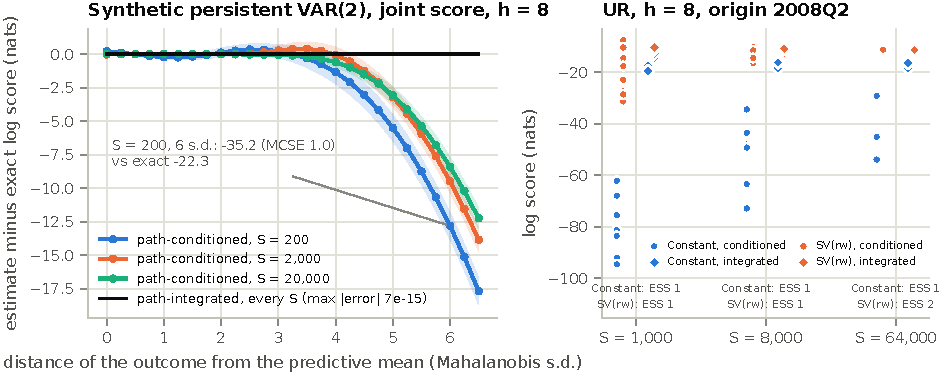
\includegraphics[width=\textwidth]{figures/fig_lpd_estimators.pdf}
  \caption{Path-conditioned (SPEC~\S7) against path-integrated (D-34) Rao--Blackwellised log
  score at $h > 1$. Left: synthetic persistent VAR(2) at $h = 8$ (one parameter draw, constant
  volatility); estimate minus the exact log score as the outcome moves from 0 to 6.5 (Mahalanobis)
  standard deviations from the predictive mean, for the conditioned estimator ($\pm$ its MCSE) with
  $S = 200$, 2000 and 20{,}000 and for the integrated one; the test's case (6 s.d., $S = 200$) is
  annotated. Right: Constant (and SV(rw)),
  unemployment, $h = 8$, origin 2008Q2, at the acceptance MCMC budget; conditioned with
  $S = 1000$, 8000 and 64{,}000 against integrated, with the spread across fit and forecast seeds
  and the weight ESS.}
  \label{fig:lpd-estimators}\label{fig:Fig4}
\end{figure}
\todo{\cref{fig:lpd-estimators}, right panel: needs \code{docs/paper/data/rb\_tail\_cell.json}
from \code{rb\_tail\_cell.py} (TODO 6); until then its numbers are recorded only (NOTES 8b).}

\paragraph{Residual error.}
The integrated estimator is still an average over draws whose weights concentrate in the tails.
A review of the estimator, recorded in the repository notes and the pre-registration of
\cref{sec:cr}, refitted the same cell at the acceptance budget ($4 \times 20{,}000$ draws): with
1000 forecast draws the Constant arm's weight ESS was 2--6, and across thinning offsets the
estimate had a standard deviation of 0.75--1.06 nats and a downward bias of about 0.3--0.6 nats;
with 8000 draws the standard deviation was 0.09--0.19 nats and the bias negligible.
% [R] main-repo docs/paper/NOTES.md 8b D-34 addendum (D-34 review, finding math-2); [PREREG] benchmarks/reports/clark_ravazzolo_preregistration.md item 3 (c823d20)
More forecast draws do not remove the MCMC error: 80{,}000-draw values still differed by about
1.3 nats across fit seeds.
% [R] same sources
The pre-registered acceptance run therefore uses 8000 forecast draws.
% [PREREG] item 3 (c823d20)

\paragraph{Scope.}
The estimator is opt-in; the SPEC default is unchanged.
It needs \code{lag\_coefs}, which MCMC forecasts of linear or zero means carry; analytic, benchmark
and ordering-pooled forecasts raise at $h > 1$, and so does combining it with
\code{rb\_transitory} at $h > 1$, which would require integrating the transitory scales of
$T+1, \dots, T+h-1$ jointly.
% [V] tests/unit/test_lpd_integrated.py::test_integrated_errors; tests/unit/test_scores_lpd_method.py::test_integrated_needs_lag_coefs_beyond_horizon_one
\todo{Risk 4: if D-34 is not on the release commit, cut the Fix and Residual-error paragraphs and
the integrated series of \cref{fig:lpd-estimators}.}

\subsection{Scores}\label{sec:eval-scores}

All scores are computed per origin, horizon and model on the transformed scale: the joint and
per-variable log score with the chosen estimator (an integrated run also stores the conditioned
values from the same forecast); the fair CRPS in its probability-weighted-moment form, computed
with \pkg{scoringrules} \citep{zanetta2024scoringrules}; quantile-weighted CRPS with centre and tail
weights \citep{gneiting2011comparing} and optional threshold-weighted CRPS; energy
\citep{gneiting2007strictly} and variogram ($p = 0.5$; \citealp{scheuerer2015variogram}) scores on
a subsample of at most 1000 draws; squared and absolute errors; and PIT values with 50\% and 90\%
coverage.
% [V] src/rai_bvar/evaluation/scores.py l.54-177 at d58c9ef; tests/unit/test_scores.py::test_unweighted_qwcrps_matches_fair_crps, ::test_crps_against_gaussian_closed_form; tests/unit/test_scores_lpd_method.py::test_integrated_layout_and_values
The log score, which is strictly proper \citep{gneiting2007strictly}, is the primary score.

\subsection{Tests of equal predictive ability}\label{sec:eval-tests}

For loss differences $d_t = \ell_{M,t} - \ell_{B,t}$ over $P$ common origins (for the log score,
$\ell = -\log\hat p$), the Diebold--Mariano statistic \citep{diebold1995comparing} uses a
rectangular-kernel long-run variance with $h - 1$ autocovariances $\hat\gamma_k$ and the
small-sample correction of \citet{harvey1997testing},
\begin{equation}\label{eq:dm}
  \mathrm{DM}_{\mathrm{HLN}} = \frac{\bar d}{\sqrt{\hat\omega/P}}
  \sqrt{\frac{P + 1 - 2h + h(h-1)/P}{P}},\qquad
  \hat\omega = \hat\gamma_0 + 2\sum_{k=1}^{h-1}\hat\gamma_k ,
\end{equation}
compared with Student-$t_{P-1}$ quantiles; Bartlett (Newey--West) weights \citep{newey1987simple}
are used only if $\hat\omega$ is not positive.
% [V] src/rai_bvar/evaluation/significance.py l.27-77 at d58c9ef; tests/unit/test_significance.py::test_dm_size_under_null, ::test_dm_hln_uses_student_t. SPEC §9.3 says Newey-West (dossier 02 §15 D1; TODO 18): the text describes the code
Following \citet{giacomini2006tests}, the package treats the $p$-values as formally valid only with
rolling or fixed windows; with expanding windows and nested models the statistic is not
asymptotically standard \citep{clark2001tests}, and the $p$-values are labelled descriptive.
% [V] tests/integration/test_compare.py::test_expanding_window_tests_are_descriptive
The test is DM with the HLN correction applied to log-score losses; \citet{amisano2007comparing}
give the analogous weighted likelihood ratio test for density forecasts.
The second route is the model confidence set \citep{hansen2011model}: the $T_{\max}$ statistic on
the joint log-score losses, with a circular block bootstrap (block length
$\max(1, \operatorname{round}(P^{1/3}))$, 2000 replications).
% [V] src/rai_bvar/evaluation/significance.py l.100-137, compare.py l.152-157 at d58c9ef; tests/unit/test_significance.py::test_mcs_eliminates_clearly_worse_models_first
Two consequences follow.
Under expanding windows a ``better'' verdict can only come through the MCS route
(\cref{sec:eval-verdict}), so results should report the route.
And the comparison table prints two-sided DM $p$-values while the verdict uses one-sided ones
(0.029 against 0.014 in \cref{lst:Lst1}).
% [V] compare.py l.172 (two-sided, table) and l.256-257 (one-sided, verdict) at d58c9ef; docs/paper/code/out/ex_a.txt

\subsection{Backtests}\label{sec:eval-backtest}

\code{backtest()} runs the origins from a start to an end date, every \code{step} periods (or a
given list of origins), with an \code{Expanding} window (tests descriptive) or a \code{Rolling}
window (tests valid).
At each origin it refits the model on the data available at that origin, cut to the window
(\code{window.select(data.upto(origin))}), so every data-dependent prior quantity is recomputed
from them (R9).
% [V] src/rai_bvar/evaluation/backtest.py l.125-137 (Origins: start, end, step) and l.412-413 at d58c9ef
% [V] tests/integration/test_backtest.py::test_no_look_ahead_and_window_sizes, ::test_results_do_not_depend_on_other_origins
Each origin has its own forecast generator and, for MCMC models, its own fit seed, both derived
from the backtest seed and the origin; a data salt keeps chains independent across windows and
orderings.
% [V] src/rai_bvar/evaluation/backtest.py l.359-370 (fit_seed) and src/rai_bvar/engines/mcmc/keys.py l.189-193 (data_salt) at d58c9ef
Scores are cached per origin under a key of spec, sample, outcomes, origin and settings, with
tags for the MCMC seeding and a non-default estimator, so runs resume and adding a model fits only
that model.
% [V] tests/integration/test_backtest.py::test_cache_roundtrip_and_invalidation; tests/integration/test_backtest_lpd_integrated.py::test_cache_keys_are_tagged_only_for_another_estimator
A pool of spawned workers reproduces the serial results to $10^{-12}$.
% [V] tests/integration/test_backtest_mcmc.py::test_spawn_pool_matches_the_serial_backtest (slow; no bitwise claim across processes)
Warm starts are opt-in and require strictly increasing origins.
% [V] src/rai_bvar/evaluation/backtest.py l.267-271 at d58c9ef

\subsection{\texorpdfstring{\code{compare()}}{compare()} and the verdict}\label{sec:eval-verdict}

\code{compare()} backtests every model on identical origins, windows and outcomes and evaluates
every statistic on the origins where all models have a finite joint log score.
For a model $M$ and a reference $B$ at horizon $h$, let $\Delta\mathrm{LPD}$ be the summed
difference of their log scores over those origins, $\mathcal D(M, B)$ the set of declared axes
(mean, prior, volatility, \dots) on which their axis labels differ,
$p_{\mathrm{DM}}$ the one-sided $p$-value of~\eqref{eq:dm} and $\mathcal M_{25\%}$ the set of
models whose MCS $p$-value is at least 0.25 (the model confidence set at $\alpha = 0.25$).
% [V] compare.py l.333-334 (_differing_axes: axis names whose labels differ) and l.259 (mcs >= mcs_alpha) at d58c9ef
The default rule is
\begin{equation}\label{eq:verdict}
\boxed{\;
\begin{aligned}
  \text{better} \iff{} & \bigl|\mathcal D(M, B)\bigr| = 1
  \;\wedge\; \Delta\mathrm{LPD} > 0
  \;\wedge\; |\Delta\mathrm{LPD}| > 3\,\mathrm{MCSE}\\
  & \wedge\; \bigl[(\text{rolling} \wedge p_{\mathrm{DM}} < 0.10)
  \;\vee\; (M \in \mathcal M_{25\%} \wedge B \notin \mathcal M_{25\%})\bigr],\\
  & \text{with } \mathrm{MCSE} = \Bigl(\textstyle\sum_t \bigl(\widehat{\mathrm{se}}_{M,t}^2
  + \widehat{\mathrm{se}}_{B,t}^2\bigr)\Bigr)^{1/2},
\end{aligned}\;}
\end{equation}
``worse'' is its mirror image, and anything else is ``inconclusive''.
% [V] src/rai_bvar/evaluation/compare.py l.202-294 (verdict), l.337-338 (MCSE in quadrature) at d58c9ef; defaults test_level=0.10, mcs_alpha=0.25, mc_multiple=3.0, min_converged=0.95
A convergence gate then forces ``inconclusive'' if either model converged at fewer than 95\% of
the origins.
% [V] compare.py l.272-281 at d58c9ef; exercised by Listing 2 (docs/paper/code/out/ex_b.txt)
\todo{No committed test calls \code{verdict(min_converged=...)} at d58c9ef; the gate is
exercised only by \cref{lst:Lst2} and the replication script. Add a unit test.}
A fit is converged when no chain raised an error, there are at least two chains, any
empirical-Bayes step converged, and every primary quantity (log-likelihood, own-first-lag
coefficients and the volatility parameters, including $h_{i,T}$ under SV) has a rank-normalised
split $\hat R$ below 1.01 and a bulk ESS above 400 \citep{vehtari2021rank}.
% [V] tests/mcmc/diagnostics/test_monitor.py::test_failure_in_a_primary_quantity_is_not_converged, ::test_low_primary_ess_is_not_converged, ::test_one_chain_is_never_converged, ::test_an_error_is_never_converged, ::test_eb_failure_is_never_converged; primary set: src/rai_bvar/engines/mcmc/monitor.py docstring (D-33)
Pairs that differ along more than one axis, or whose specs differ without a declared axis, are
``not comparable''.
% [V] tests/integration/test_compare.py::test_two_axis_differences_are_not_comparable, ::test_identical_models_are_inconclusive
With \code{verdict(axis="vol")} each model is paired with the arm that has the baseline's value on
that axis and agrees on all others, and \code{grid()} harmonises the arms so that this pairing is
meaningful: in a volatility grid the Constant baseline becomes the MCMC Mode~I model
\code{Constant("ig")}, not the analytic NIW model, and Mode~II is labelled a prior change.
% [V] tests/unit/test_grid_harmonise.py::test_spec_grid_becomes_a_one_axis_volatility_comparison, ::test_mode_one_and_mode_two_arms_are_named_apart
\cref{fig:verdict-flow} shows the rule as a decision flow.
Each ingredient is standard; their combination into one automatic rule is the package's.
The rule's size and power have not been studied, and the quadrature MCSE treats the two models'
errors as independent although both use the same per-origin forecast seed
(\cref{sec:limitations}).
% dossier 02 §15 D4 and Q4; no tests/dgp/ (SPEC §10.5); TODO 10

\begin{figure}[tbp]
  \centering
  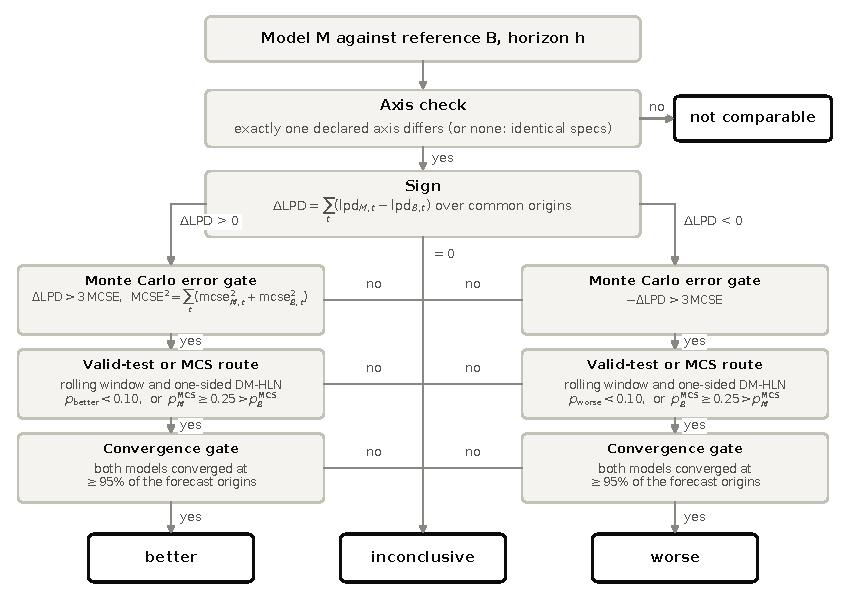
\includegraphics[width=0.85\textwidth]{figures/fig_verdict_flow.pdf}
  \caption{The verdict rule~\eqref{eq:verdict} as a decision flow: axis check, sign, Monte Carlo
  error gate, valid-test or MCS route, convergence gate. The outcomes are better, worse,
  inconclusive and not comparable.}
  \label{fig:verdict-flow}\label{fig:Fig3}
\end{figure}

\subsection{Ordering sensitivity}\label{sec:eval-ordering}

In general, a composition with a triangular factorisation depends on the variable ordering,
through the prior or through the model class \citep{arias2023macroeconomic,chan2024large}.
The check (\code{rb.ordering\_sensitivity()}) re-evaluates a model under all, Latin-square-balanced
or random permutations of the variables: in prior mode it simulates the prior under each ordering
without a fit, and in forecast or backtest mode it refits, recomputing every data-dependent quantity
from the permuted window.
A metric such as the range of log scores over orderings is flagged only when it exceeds its
threshold (0.05 nats per variable, 0.10 joint) and its signal-to-noise ratio against the noise
floor $\sigma_{\mathrm{MC}} = \max(\text{sd across seeds}, \text{MCSE})$ exceeds 3.
% [V] src/rai_bvar/structural/ordering.py module docstring and THRESHOLDS (l.113-121) at d58c9ef; tests/integration/test_ordering.py
Optionally, the check returns the equal-weight mixture over orderings, which is exactly
order-invariant when all orderings are used.
% [V] src/rai_bvar/structural/ordering.py module docstring (pool=True) at d58c9ef
MCMC fits of compositions that are not order-invariant warn from $n = 4$ variables on (R8).
% [V] src/rai_bvar/engines/mcmc/monitor.py l.77 (_ORDERING_N = 4), l.692-699 at d58c9ef
Besides the analytic NIW engine, the only order-invariant composition in Phase~2 is the MCMC model
reduced form $\times$ \code{Constant("iw\_equivalent")}, whose implied $\Sigma$ prior is inverse
Wishart \citep{chan2022asymmetric}.
That model is the Constant arm of the replication, where it serves as a negative control for the
ordering check (\cref{sec:cr}; see \cref{sec:limitations} for how the check treated it in the
first full run).
% [V] src/rai_bvar/structural/ordering.py l.5-7 at d58c9ef; [PREREG] benchmarks/reports/clark_ravazzolo_preregistration.md "What does not change" (Models: Constant(iw_equivalent), reduced-form mean prior); first-run flag: dossier 02 §10.3 fact-check note, OUTLINE risk 16
% [V] tests/integration/test_ordering.py::test_analytic_engine_is_exactly_order_invariant; ::test_reduced_iw_equivalent_is_order_invariant_within_mcse (slow)
